\documentclass[11pt, oneside]{amsart}

\usepackage[utf8]{inputenc}

\usepackage{amsfonts, amstext, amsmath, amsthm, amscd, amssymb}
\usepackage{mathrsfs}
\usepackage{tikz}
\usetikzlibrary{knots}
\tikzset{point/.style={insert path={ node[scale=2.5*sqrt(\pgflinewidth)]{.} }}}
\usepackage{url}
\usepackage[all]{xypic}

\usepackage{color}
\usepackage[colorlinks,
    linkcolor={red!50!black},
    citecolor={blue!50!black},
    urlcolor={blue!80!black}]{hyperref}

\usepackage{enumerate}

   
 
 

\numberwithin{equation}{section}

\theoremstyle{plain}
\newtheorem{theorem}[equation]{Theorem}
\newtheorem{lemma}[equation]{Lemma}
\newtheorem{proposition}[equation]{Proposition}
\newtheorem{property}[equation]{Property}
\newtheorem{corollary}[equation]{Corollary}
\newtheorem*{fact}{fact}

\newtheorem{conjecture}[equation]{Conjecture}
\newtheorem{thm}[equation]{Theorem}
\newtheorem{cor}[equation]{Corollary}
\newtheorem{lem}[equation]{Lemma}
\newtheorem{prop}[equation]{Proposition}

\newtheorem{convention}{Convention}

\theoremstyle{definition}
\newtheorem{example}[equation]{Example}
\newtheorem{exercise}[equation]{Exercise}
\newtheorem{definition}[equation]{Definition}
\newtheorem{problem}[equation]{Problem}
\newtheorem{conventions}[equation]{Conventions}
\newtheorem{remark}[equation]{Remark}

\theoremstyle{remark}
\newtheorem*{claim}{Claim}

\newtheorem*{ack}{Acknowledgements}

\numberwithin{equation}{section}

\begin{document}

\title{The round handle problem}

\author{Min Hoon Kim}
\address{School of Mathematics, KIAS, Seoul, Republic of Korea}
\email{kminhoon@gmail.com}

\author{Mark Powell}
\address{D\'epartement de Math\'ematiques,
Universit\'e du Qu\'ebec \`a Montr\'eal, Canada}
\email{mark@cirget.ca}

\author{Peter Teichner}
\address{Max Planck Institut f\"{u}r Mathematik, Vivatsgasse 7, 53111 Bonn, Germany}
\email{teichner@mpim-bonn.mpg.de}

\expandafter\let\csname subjclassname@1991\endcsname={\textup{2010} Mathematics Subject Classification}
\expandafter\let\csname subjclassname@2000\endcsname={\textup{2010} Mathematics Subject Classification}
\subjclass{ 57M25, 
 57M27, 
  57N13, 
 57N70, 
}
\keywords{Round handle problem, topological surgery, $s$-cobordism}

\begin{abstract}
We present the Round Handle Problem (RHP), proposed by Freedman and Krushkal. It asks whether a collection of links, which contains the Generalised Borromean Rings (GBRs), are slice in a $4$-manifold $R$ constructed from adding round handles to the four ball.  A negative answer would contradict the union of the surgery conjecture and the $s$-cobordism conjecture for $4$-manifolds with free fundamental group.
\end{abstract}

\maketitle

\section{Statement of the RHP}

These notes give an alternative proof of the connection of the Round Handle Problem to the topological surgery and $s$-cobordism conjectures (these will all be recalled below).  The Round Handle Problem (RHP) was formulated in \cite[Section~5.1]{Freedman-Krushkal-2016-A}.  We give a shorter and easier argument that the above mentioned conjectures imply a positive answer to the RHP.

Let $L = L_1 \sqcup \cdots \sqcup L_m$ be an oriented ordered link in $S^3$ with vanishing pairwise linking numbers.  We will be particularly concerned with the Generalised Borromean Rings (GBRs). By definition these are the collection of links arising from iterated Bing doubling starting with a Hopf link.

Write $X_L := S^3 {{\smallsetminus}} \nu L$ for the exterior of $L$.
Let $\mu_{i} \subset X_L$ be an oriented meridian of the $i$th component of $L$, and let $\lambda_i \subset X_L$ be a zero-framed oriented longitude.  Make $\mu_i$ small enough that $\operatorname{lk}(\mu_i,\lambda_i)=0$  (of course $\operatorname{lk}(\mu_i,L_i) =1$ and $\operatorname{lk}(\lambda_i,L_i)=0$).

A \emph{Round handle} $H$ is a copy of $S^1 \times D^2 \times D^1$.  The \emph{attaching region} is $S^1 \times D^2 \times S^0 \subset \partial(S^1 \times D^2 \times D^1) \cong S^1 \times S^2$.

\begin{definition}
  Given an $m$-component link $L$, construct a manifold $R(L)$ by attaching $m$ round handles $\{H_i\}_{i=1}^m$ to $D^4$ as follows.  For the $i$th round handle, glue $S^1 \times D^2 \times \{-1\}$ to $\nu \mu_i \subset X_L \subset S^3= \partial D^4$, and glue $S^1 \times D^2 \times \{1\}$ to $\nu \lambda_i$.  In both cases use the zero-framing for the identification of $\nu \mu_i$ and $\nu \lambda_i$ with $S^1 \times D^2$.
  Note that the link $L$ lies in $\partial R(L)$.
\end{definition}

\noindent The key question will be whether $L$ is slice in $R(L)$.

\begin{definition}[Round Handle Slice]
  A link $L$ is \emph{Round Handle Slice (RHS)} if $L \subset \partial R(L)$ is slice in $R(L)$, that is if $L$ is the boundary of a disjoint union of locally flat embedded discs in $R(L)$.
\end{definition}

\begin{theorem}\label{theorem:RHP}
Suppose that the topological surgery and $s$-cobordism conjectures hold.  Then for any link $L$ with pairwise linking numbers all zero, $L$ is round handle slice.
\end{theorem}

\begin{problem}
The Round Handle Problem is to determine whether all pairwise linking number zero links are slice in $R(L)$.
\end{problem}

A negative answer for one such link would contradict the logical union of the topological surgery conjecture and the $s$-cobordism conjecture.
We briefly recall the statements of these conjectures.

\begin{conjecture}[Topological surgery conjecture]
  Any degree one normal map $(M,\partial M) \to (X,\partial X)$ from a $4$-manifold $M$ to a $4$-dimensional Poincar\'{e} pair $(X,\partial X)$, that is a ${\mathbb Z}[\pi_1(X)]$-homology equivalence on the boundary, is topologically normally bordant rel.\ boundary to a homotopy equivalence if and only if the surgery obstruction in $L_4({\mathbb Z}[\pi_1(X)])$ vanishes.
\end{conjecture}

\begin{conjecture}[$s$-cobordism conjecture]
   Every compact topological $5$-dimensional $s$-cobordism $(W;M_0,M_1)$, that is a product on the boundary, is homeomorphic to a product $W \cong M_0 \times I \cong M_1 \times I$, extending the given product structure on the boundary.
\end{conjecture}

It is suggested by Freedman and Krushkal, but by no means compulsory, to focus on the links arising as GBRs.
It is also suggested that one might try to adapt Milnor's invariants to provide obstructions.
The primary purpose of this problem, like the AB slice problem, is to provide a way to get obstructions to surgery and $s$-cobordism.

\subsection*{Acknowledgements}

We thank Allison N.\ Miller for delivering an excellent lecture on the Round Handle Problem, that motivated us to produce this alternative proof.
We also are extremely grateful to the Hausdorff Insititute for Mathematics in Bonn, in whose fantastic research environment these notes were written.

\section{Proof of Theorem~\ref{theorem:RHP}}

The proof of Theorem~\ref{theorem:RHP} involves the construction of an $s$-cobordism rel.\ boundary from the manifold $R(L)$, henceforth abbreviated to $R$, to another $4$-manifold $R'$, in which $L$ is slice.

We begin with a Kirby diagram for $R$, shown in Figure~\ref{figure:RHP1}.
First we will explain the figure, then we will explain why this is a diagram for $R$.  The diagram does not show the literal Kirby diagram for $R$.  Rather, the curve labelled $d$ specifies a solid torus, as the complement of a regular neighbourhood of this curve.  Inside the solid torus two dotted circles, corresponding to 1-handles, and two zero-framed circles, corresponding to $2$-handles, can be seen.  Embed a copy of this solid torus into $\nu L_i$ for each $i=1,\dots,m$ using the zero framing.    The diagram also shows the link $L$ parallel to the core of the solid torus.

\begin{figure}[htb]
\centering
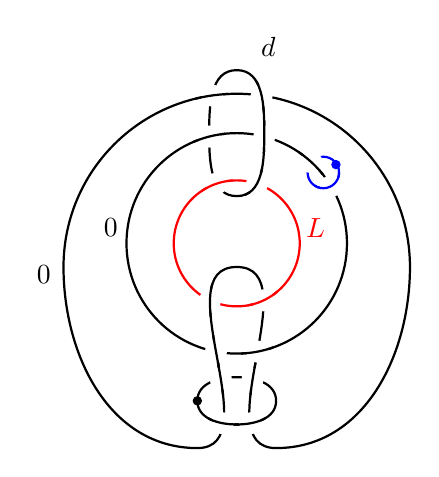
\begin{tikzpicture}
\begin{knot}[
clip width=10, clip radius=4pt,ignore endpoint intersections=false,]

\strand[thick] (3.2,0.3)
to [out=up, in=right] (1,2.5)
to [out=left, in=up] (-1.2,0.3)
to [out=down, in=left] (0.5,-2)
to [out=right, in=left] (1,0.3)
to [out=right, in=left] (1.5,-2)
to [out=right, in=down] (3.2,0.3);

\strand[thick]
(0.5,-1.4)
to [out=up,in=left] (1,-1.1)
to [out=right, in=up] (1.5,-1.4)
to [out=down, in=right] (1,-1.7)
to [out=left, in=down] (0.5,-1.4);

\strand[thick,color=red]
(1,-0.2)
to [out=right, in=down] (1.8,0.6)
to [out=up, in=right] (1,1.4)
to [out=left, in=up] (0.2,0.6)
to [out=down,in=left] (1,-0.2);

\strand[thick]
(1,-0.8)
to [out=right, in=down] (2.4,0.6)
to [out=up, in=right] (1,2)
to [out=left, in=up] (-0.4,0.6)
to [out=down,in=left] (1,-0.8);

\strand[thick]
(1,1.2)
to [out=right, in=down] (1.35,2)
to [out=up, in=right] (1,2.8)
to [out=left, in=up] (0.65,2)
to [out=down, in=left] (1,1.2);

\strand[thick,color=blue]
(2.1,1.3)
to [out=right, in=down] (2.3,1.5)
to [out=up, in=right] (2.1,1.7)
to [out=left, in=up] (1.9, 1.5)
to [out=down, in=left] (2.1,1.3);

\draw[color=black] (1.4,3.1) node {$d$};
\draw[color=black] (-0.6,0.8) node {$0$};
\draw[color=black] (-1.45,0.2) node {$0$};
\fill[color=blue] (2.26,1.6)  circle[radius=1.7pt];
\fill[color=black] (0.5,-1.4)  circle[radius=1.7pt];
\draw[color=red] (2,0.8) node {$L$};
\flipcrossings{2,4,6,8,9,11,13,15}
\end{knot}
\end{tikzpicture}
\caption{A handle diagram for $R$.}
\label{figure:RHP1}

\end{figure}

Now we explain why Figure~\ref{figure:RHP1} is a diagram for the $4$-manifold $R$.
Observe that one of the 1-handles and one of the 2-handles are in cancelling position.  Cancel this pair, to obtain the handle diagram shown in Figure \ref{figure:RHP2}.
This diagram which can be seen with a little thought to be a diagram for $R$.  A round handle can be constructed from a 1-handle and a 2-handle whose boundary goes around one attaching circle of the round handle (a meridian of $L$), traverses the 1-handle, goes around the other attaching circle (a zero-framed longitude of the same component of $L$), and then traverses the $1$-handle in the other direction.   Ignoring the link $L$, we see that $R$ is diffeomorphic to the zero-trace of $L$ with $m$ $1$-handles added.

\begin{figure}[htb]
\centering
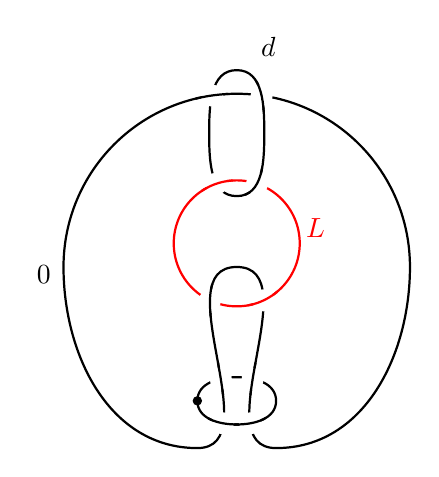
\begin{tikzpicture}
\begin{knot}[
clip width=10, clip radius=4pt,ignore endpoint intersections=false,]

\strand[thick] (3.2,0.3)
to [out=up, in=right] (1,2.5)
to [out=left, in=up] (-1.2,0.3)
to [out=down, in=left] (0.5,-2)
to [out=right, in=left] (1,0.3)
to [out=right, in=left] (1.5,-2)
to [out=right, in=down] (3.2,0.3);

\strand[thick]
(0.5,-1.4)
to [out=up,in=left] (1,-1.1)
to [out=right, in=up] (1.5,-1.4)
to [out=down, in=right] (1,-1.7)
to [out=left, in=down] (0.5,-1.4);

\strand[thick,color=red]
(1,-0.2)
to [out=right, in=down] (1.8,0.6)
to [out=up, in=right] (1,1.4)
to [out=left, in=up] (0.2,0.6)
to [out=down,in=left] (1,-0.2);

\strand[thick]
(1,1.2)
to [out=right, in=down] (1.35,2)
to [out=up, in=right] (1,2.8)
to [out=left, in=up] (0.65,2)
to [out=down, in=left] (1,1.2);

\draw[color=black] (1.4,3.1) node {$d$};
\draw[color=black] (-1.45,0.2) node {$0$};
\fill[color=black] (0.5,-1.4)  circle[radius=1.7pt];
\draw[color=red] (2,0.8) node {$L$};
\flipcrossings{2,4,6,7,9}
\end{knot}
\end{tikzpicture}
\caption{The diagram for $R$ from Figure~\ref{figure:RHP1} after cancellations.}
\label{figure:RHP2}

\end{figure}

Next, Figure~\ref{figure:RHP3} shows a Kirby diagram, with the same convention as above, for a 4-manifold that we call $R_M$.  Here $M$ stands for ``middle,'' since this manifold will lie in the middle of an $s$-cobordism that we are about to construct.

\begin{figure}[htb]
\centering
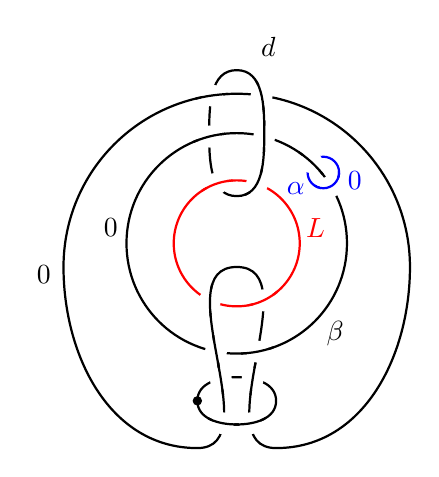
\begin{tikzpicture}
\begin{knot}[
clip width=10, clip radius=4pt,ignore endpoint intersections=false,]

\strand[thick] (3.2,0.3)
to [out=up, in=right] (1,2.5)
to [out=left, in=up] (-1.2,0.3)
to [out=down, in=left] (0.5,-2)
to [out=right, in=left] (1,0.3)
to [out=right, in=left] (1.5,-2)
to [out=right, in=down] (3.2,0.3);

\strand[thick]
(0.5,-1.4)
to [out=up,in=left] (1,-1.1)
to [out=right, in=up] (1.5,-1.4)
to [out=down, in=right] (1,-1.7)
to [out=left, in=down] (0.5,-1.4);

\strand[thick,color=red]
(1,-0.2)
to [out=right, in=down] (1.8,0.6)
to [out=up, in=right] (1,1.4)
to [out=left, in=up] (0.2,0.6)
to [out=down,in=left] (1,-0.2);

\strand[thick]
(1,-0.8)
to [out=right, in=down] (2.4,0.6)
to [out=up, in=right] (1,2)
to [out=left, in=up] (-0.4,0.6)
to [out=down,in=left] (1,-0.8);

\strand[thick]
(1,1.2)
to [out=right, in=down] (1.35,2)
to [out=up, in=right] (1,2.8)
to [out=left, in=up] (0.65,2)
to [out=down, in=left] (1,1.2);

\strand[thick,color=blue]
(2.1,1.3)
to [out=right, in=down] (2.3,1.5)
to [out=up, in=right] (2.1,1.7)
to [out=left, in=up] (1.9, 1.5)
to [out=down, in=left] (2.1,1.3);

\draw[color=black] (1.4,3.1) node {$d$};
\draw[color=black] (-0.6,0.8) node {$0$};
\draw[color=black] (-1.45,0.2) node {$0$};
\draw[color=blue] (1.75,1.3) node{$\alpha$};
\draw[color=blue] (2.5,1.4) node{$0$};
\draw[color=black] (2.25,-0.55) node{$\beta$};
\fill[color=black] (0.5,-1.4)  circle[radius=1.7pt];
\draw[color=red] (2,0.8) node {$L$};
\flipcrossings{2,4,6,8,9,11,13,15}
\end{knot}
\end{tikzpicture}
\caption{A handle diagram for $R_M$.}
\label{figure:RHP3}
\end{figure}

The diagram for $R_M$ is very similar to the diagram for $R$ from Figure~\ref{figure:RHP1}; in order to get from the diagram for $R_M$ to that for $R$, change the zero-framed 2-handle whose attaching curve is labelled $\alpha$ in Figure~\ref{figure:RHP3} to a 1-handle. That is, perform surgery on the 2-sphere obtained from the core of the 2-handle union a disc bounded by the attaching circle in $D^4$.  Note that, by virtue of the cores of the $2$-handle labelled $\beta$ in Figure~\ref{figure:RHP3}, $L$ is slice in $R_M$.  To see this, just observe that $L$ can be passed through the attaching region of the $\alpha$ $2$-handles in Figure~\ref{figure:RHP3}.  On the other hand, in Figure~\ref{figure:RHP1}, $L$ cannot be passed through a dotted circle corresponding to a $1$-handle, so this argument cannot be used to show that $L$ is slice in $R$ in Figure~\ref{figure:RHP1}.  If one passes the link past the attaching region of a $2$-handle, one cannot later use the core of that $2$-handle to construct an embedded slice disc.  So likewise one cannot use Figure~\ref{figure:RHP2} to see that~$L$ is slice in~$R$.

On the other hand, there are also immersed 2-spheres in $R_M$ obtained from the union of the cores of the $\beta$ 2-handles with immersed discs in $D^4$ bounded by the $\beta$ attaching curves.  The linking number zero hypothesis implies that the algebraic intersection numbers between these 2-spheres vanish.
These $\beta$ spheres have framed dual spheres arising from the round handle $2$-handles; namely the $2$-handles that also appear in Figure~\ref{figure:RHP2}.  These 2-handles are algebraically dual to the $\beta$ spheres because they have attaching curves that link the $\beta$ curves once.

    Assuming the topological surgery conjecture, we can therefore find embedded spheres representing the regular homotopy classes of the $\beta$ 2-spheres.  We apply the disc embedding theorem in the complement of the slice discs for $L$ in $R_M$.  Define $R'$ to be the $4$-manifold obtained as result of these surgeries.
Note that $L$ is still slice in $R'$, since our initial immersed discs and their duals lie in the complement of the slice discs, and we apply the disc embedding theorem in this complement.  We are assuming that the disc embedding theorem holds for all fundamental groups, so we do not need to control the fundamental group here.

\begin{lemma}
  The $4$-manifolds $R$ and $R'$ are $s$-cobordant rel.\ boundaries.
\end{lemma}

\begin{proof}
  Start with $R_M$.  The trace of surgeries on the $\alpha$ spheres gives a cobordism to $R$.  The trace of surgeries on the $\beta$ spheres gives a cobordism to $R'$.  The union of the two cobordisms along $R_M$ is an $s$-cobordism from $R$ to $R'$, since algebraically the intersection numbers $\alpha_i \cdot \beta_j = \delta_{ij}$.
\end{proof}

Note that we used duals to the $\beta$ spheres twice, once to apply surgery and once to prove that we have an $s$-cobordism. However we use \emph{different} duals.  For the surgery we use the duals arising from the round handle $2$-handles.  For the $s$-cobordism, we use the $\alpha$ spheres.

Then since $R$ and $R'$ are $s$-cobordant, the $s$-cobordism conjecture implies that they are homeomorphic.  The homeomorphism is an identity on the boundary, so preserves the link $L$.  Thus the image of the slice discs for $L$ in $R'$ under the homeomorphism $f \colon R' \to R$ are slice discs for $L$ in~$R$.  It follows that $L$ is Round Handle Slice as desired.
This completes the proof of Theorem~\ref{theorem:RHP}.

\bibliographystyle{alpha}

\bibliography{research}
\end{document}

